\documentclass{article}

\usepackage[T1]{fontenc}
\usepackage[utf8]{inputenc}
\usepackage[brazilian]{babel}
\usepackage{graphicx}
\usepackage[export]{adjustbox}[2011/08/13]
\usepackage{float}
\usepackage[pdftex]{hyperref}
\usepackage{epstopdf}
\usepackage{etoolbox}
\usepackage{amsmath}
\usepackage{amsfonts}
\usepackage{amssymb}
\usepackage{caption}
\usepackage{subcaption}
\usepackage{setspace}
\usepackage{tikz}
\usepackage{listings}
\usepackage{xcolor} 

\bibliographystyle{eric}
\patchcmd{\thebibliography}{\section*}{\section}{}{}


\newcommand{\R}{\ensuremath{\mathbb{R}}}
\newcommand{\Prob}{\ensuremath{\mathbb{P}}}
\newcommand{\K}{\ensuremath{\mathbb{K}}}
\newcommand{\U}{\ensuremath{\mathbb{U}}}
\newcommand{\N}{\ensuremath{\mathbb{N}}}
\newcommand{\Lg}{\ensuremath{\mathbb{L}}}
\newcommand{\T}{\ensuremath{\rm Tr}}
\newcommand{\sg}{{\sigma(x_k)}}

\newcommand{\G}{\ensuremath{\mathcal{G}}}
\newcommand{\F}{\ensuremath{\mathcal{F}}}
\newcommand{\C}{\ensuremath{\mathcal{C}}}
\newcommand{\E}{\ensuremath{\mathcal{E}}}
\newcommand{\Hn}{\ensuremath{\mathcal{H}}}
\newcommand{\Hoo}{\ensuremath{\mathcal{H}_\infty}}
\newcommand{\Hop}{\ensuremath{\mathcal{H}_{op}}}
% --------------------------------------------------
\newtheorem{theo}{Teorema}
\newtheorem{exa}{Exemplo}
\newtheorem{lemm}{Lema}
\newtheorem{coro}{Corolário}
\newtheorem{defn}{Definição}[section]

\begin{document}

\begin{titlepage}
\begin{center}

\newcommand{\HRule}{\rule{\linewidth}{0.5mm}}
% Upper part of the page. The '~' is needed because \\
% only works if a paragraph has started.

\includegraphics[width=0.15\textwidth]{logoUnicamp}~\\[1cm]

\textsc{\LARGE Universidade Estadual de Campinas}\\[1.5cm]

\textsc{\Large Faculdade de Engenharia Mecânica}\\[0.5cm]

% Title
\HRule \\[0.4cm]
{ \huge \bfseries ES664 - Laboratório de Eletrônica para Automação Industrial\\ \vspace{1cm} Relatório - Experimento 4\\
\Large{Acionamento de motor DC} \\[0.4cm] }

\HRule \\[1.5cm]

% Author and supervisor
\begin{minipage}{0.6\textwidth}
\begin{flushleft} \large
\emph{Nome:}\\
Daniel Dello Russo Oliveira\\Marcelli Tiemi Kian
\end{flushleft}
\end{minipage}
\begin{minipage}{0.2\textwidth}
\begin{flushright} \large
\emph{RA}\\ 101918\\117892
\end{flushright}
\end{minipage}

\vfill

% Bottom of the page
{\large \today}

\end{center}
\end{titlepage}


\onehalfspacing
\section{Objetivos}
	Essa simulação tem como objetivo o estudo dos motores de indução assíncrono trifásico e seu acionamento através da estratégia de controle V-Hz.
	 
\section{Simualações}
Utilizamos o bloco AC2 do Simulink para simular a estratégia de controle V-Hz para um motor AC. Ajustamos os parâmetros do motor de acordo com o roteiro e conectamos a saída de medição da corrente em uma fase do estator a um bloco PLL para medição de frequência, afim de determinar a frequência síncrona do motor e consequentemente o slip. A entrada do bloco AC2 foi uma velocidade de referência constante de $1500 rpm$ e um degrau no torque de referência que varia de $1$ para $5.5 N\cdot m$ no segundo 6. O esquema da simulação está apresentado na figura \ref{fig:sim1}.
\begin{figure}[H]
	\centering
	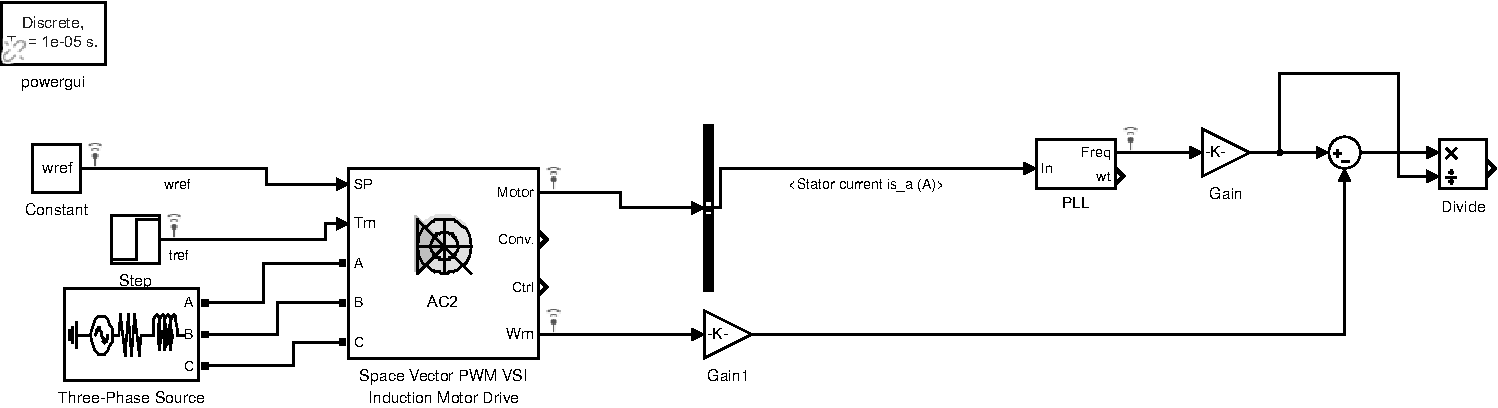
\includegraphics[width=\linewidth]{matlab/sim1}
	\caption{Esquemático da primeira simulação}
	\label{fig:sim1}
\end{figure}

%TODO citar alguem \cite{bb:mohan} ?
Para o cálculo do slip do motor sabemos que:
\begin{equation}
	s = \frac{n_s - n_r}{ns}
\end{equation}
Onde $n_s$ é a velocidade síncrona (velocidade do campo magnético) e $n_r$ é a velocidade do rotor.
Sabemos também que:
\begin{equation}
	n_s = \frac{2f}{p}
\end{equation}
Onde $p$ é o número de pólos e $f$ é a frequência da corrente elétrica passando pelo estator (devemos lembrar que essa não é a mesma frequência de nossa fonte pois no controle V-Hz utilizamos um inversor de frequência). Encontramos então $f$ medindo a frequência da corrente de uma fase no estator através de um bloco PLL (ao comparar a curva de saída do PLL e a curva de referência em frequência do controlador vimos que as duas são praticamente idênticas então acreditamos que o bloco está configurado corretamente).

Simulamos nosso sistema e encontramos as curvas de corrente na fase A no estator, torque eletromagnético e velocidade no rotor (comparando com o sinal de referência de entrada e do controlador) e a curva que relaciona o torque eletromagnético com o escorregamento, conforme pode ser visto na figura \ref{fig:s1}
\begin{figure}[H]
	\centering
	\begin{subfigure}[b]{0.49\linewidth}
		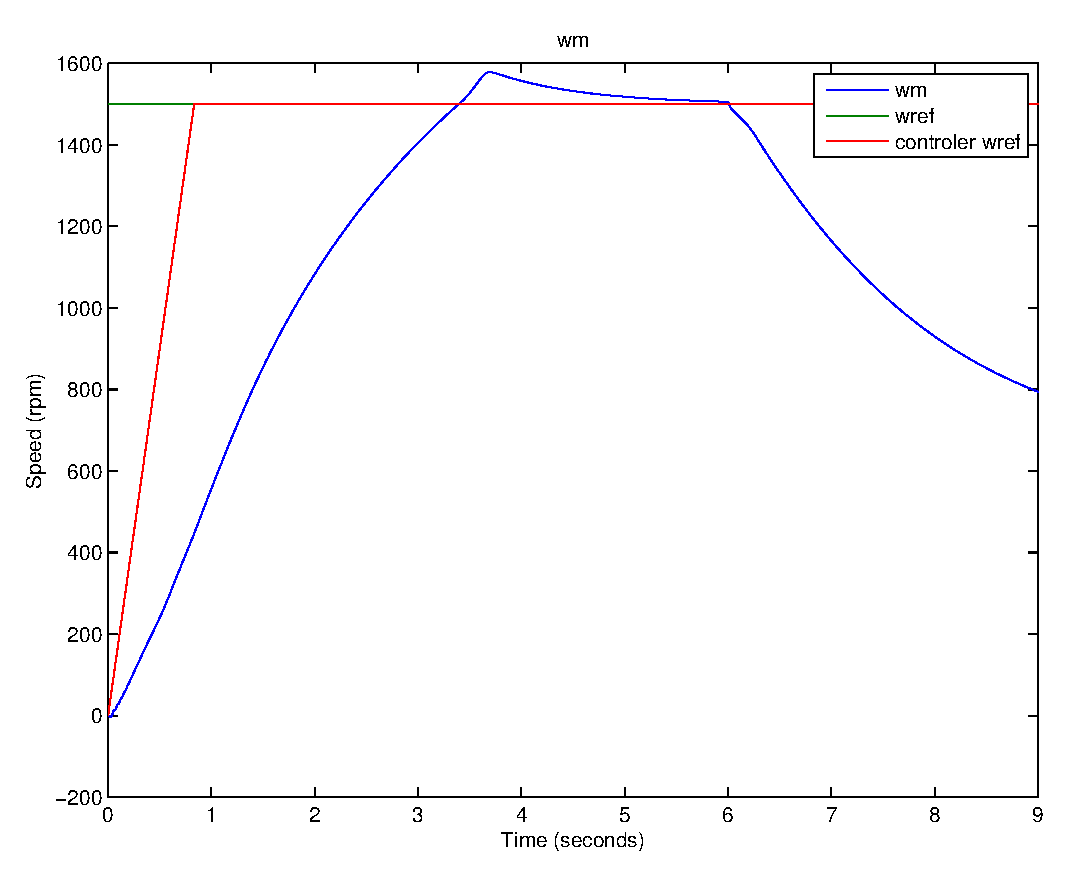
\includegraphics[width=\linewidth]{matlab/wm}
		\caption{Velocidade Angular}
	\end{subfigure}
	\begin{subfigure}[b]{0.49\linewidth}
		\centering
		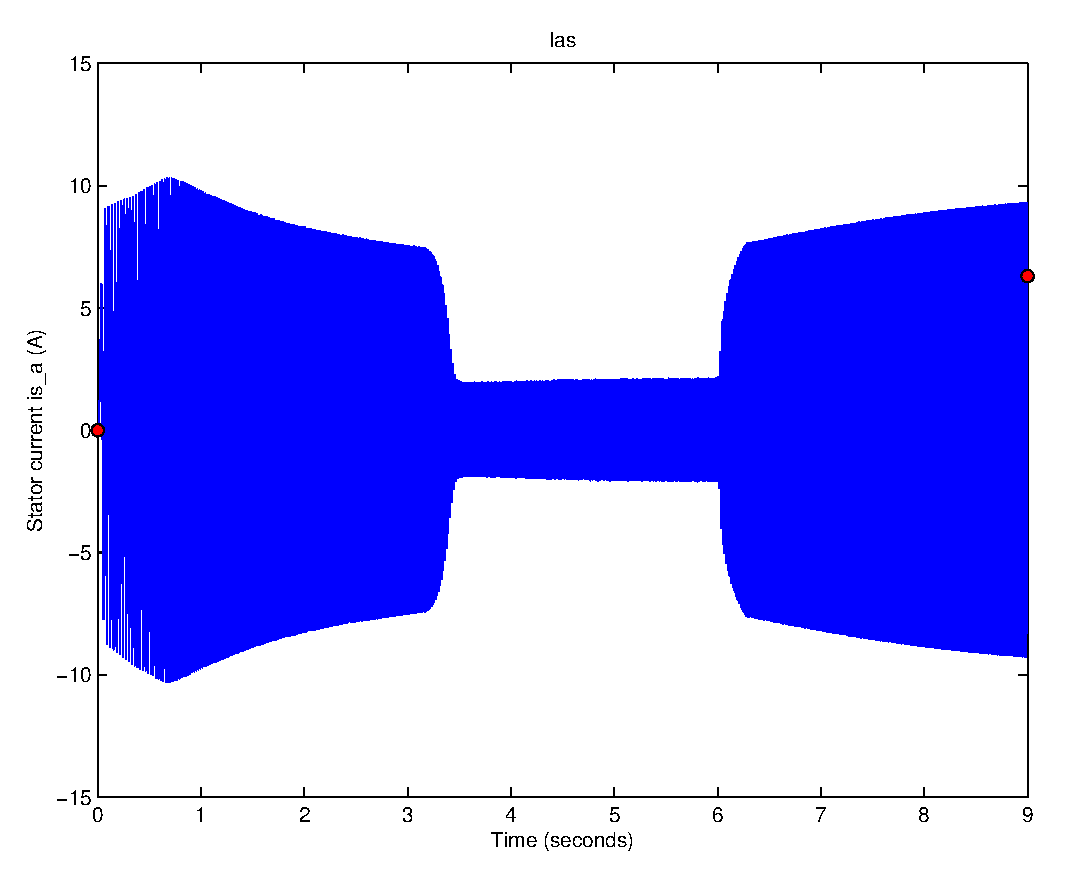
\includegraphics[width=\linewidth]{matlab/ias}
		\caption{Corrente no estator}
	\end{subfigure}
	\begin{subfigure}[b]{0.49\linewidth}
		\centering
		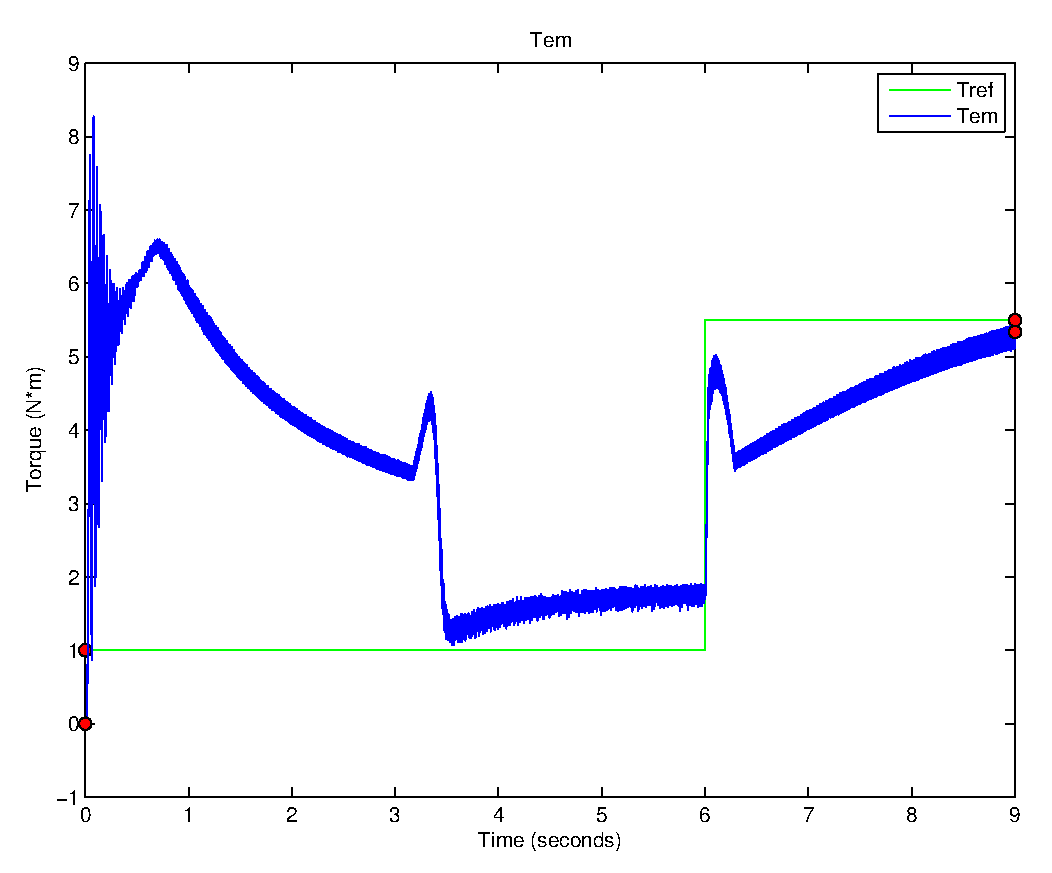
\includegraphics[width=\linewidth]{matlab/tem}
		\caption{Torque eletromagnético}
	\end{subfigure}
		\begin{subfigure}[b]{0.49\linewidth}
			\centering
			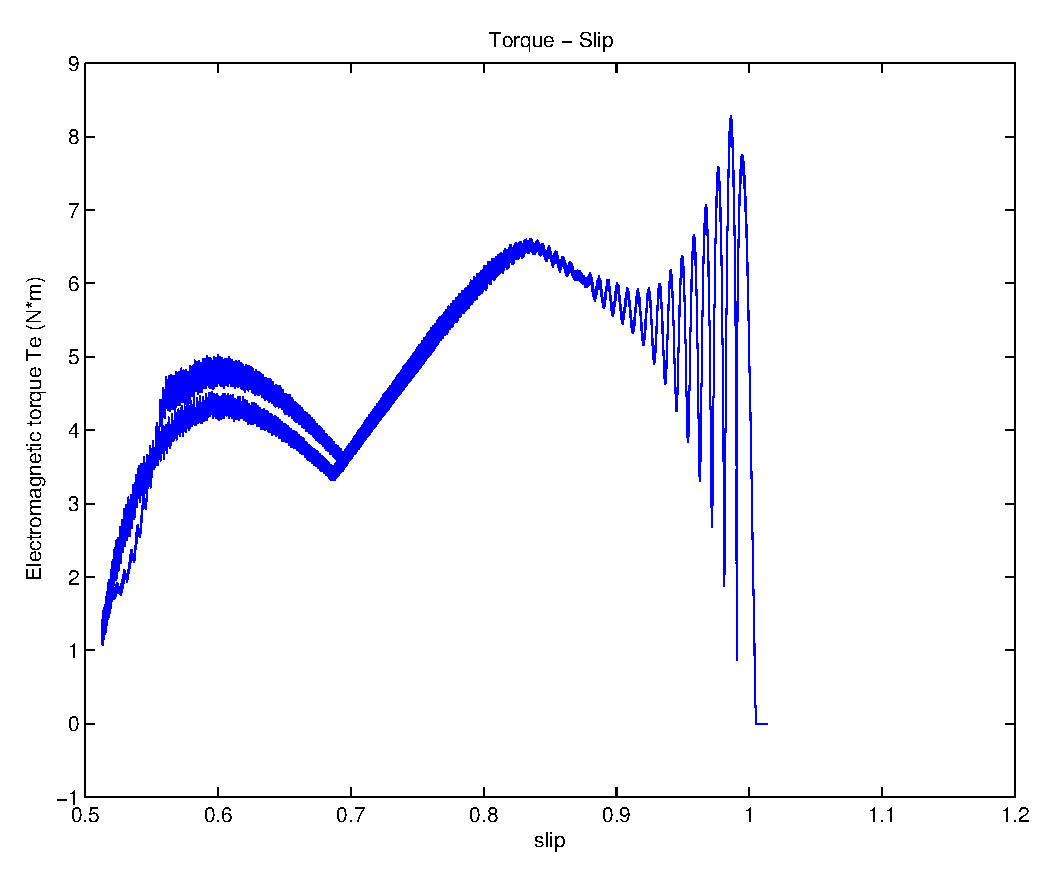
\includegraphics[width=\linewidth]{matlab/ts}
			\caption{Torque em função do slip}
		\end{subfigure}
	\caption{Curvas de resposta para primeira simulação}
	\label{fig:s1}
\end{figure}

Podemos ver que o controle apresentou um resultado não muito agradável. Ao controlar isoladamente a velocidade do motor conseguimos atingir o valor desejado em aproximadamente 4 segundos, nessa marca também ajustamos o torque para que ele se aproxime do torque desejado. Porém ao mudar a referência de torque, nosso controlador não foi capaz de manter a curva de velocidade no valor desejado enquanto perseguia o degrau no torque. Devemos levar em consideração que o controlador apresentado não foi dimensionado para o motor simulado, fator que afeta sua performance, uma vez que alteramos os parâmetros do motor sem mexer no controlador.

%TODO falar do slip, entender graficos

Mudamos então os sinais de referência para uma rampa que se inicializa no segundo $1$ e vai de $0$ a $1500 rpm$ em 3 segundos para a velocidade e um degrau de vai de $0$ para $1 N \cdot m$ no segundo 6 para o torque, conforme apresentado na figura \ref{fig:sim2}.

\begin{figure}[H]
	\centering
	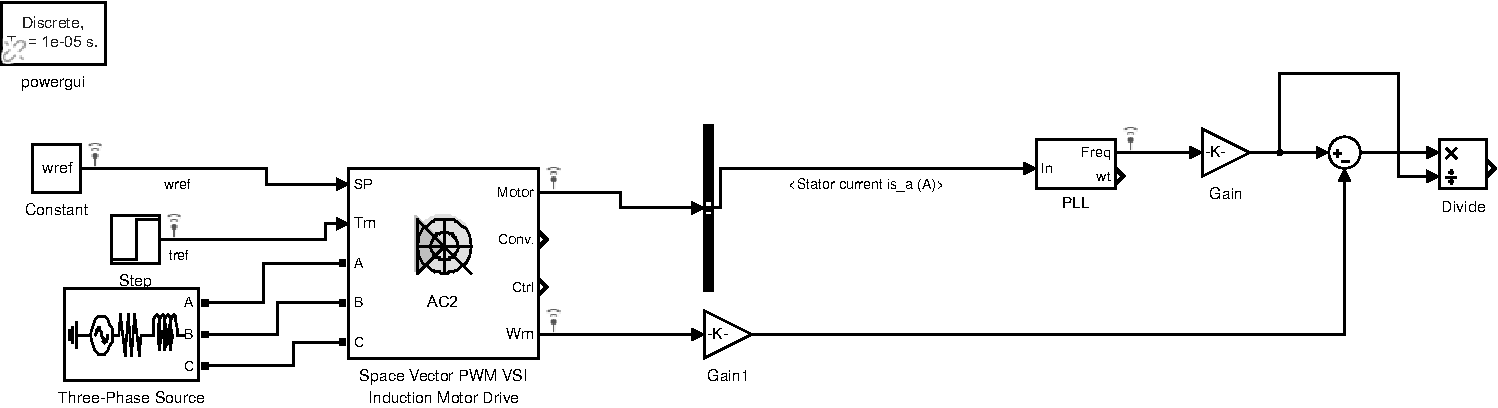
\includegraphics[width=\linewidth]{matlab/sim1}
	\caption{Esquemático da segunda simulação}
	\label{fig:sim2}
\end{figure}

Simulamos nosso sistema e encontramos as curvas de corrente na fase A no estator, torque eletromagnético e velocidade no rotor (comparando com o sinal de referência de entrada e do controlador) e a curva que relaciona o torque eletromagnético com o escorregamento, conforme pode ser visto na figura \ref{fig:s2}

\begin{figure}[H]
	\centering
	\begin{subfigure}[b]{0.49\linewidth}
		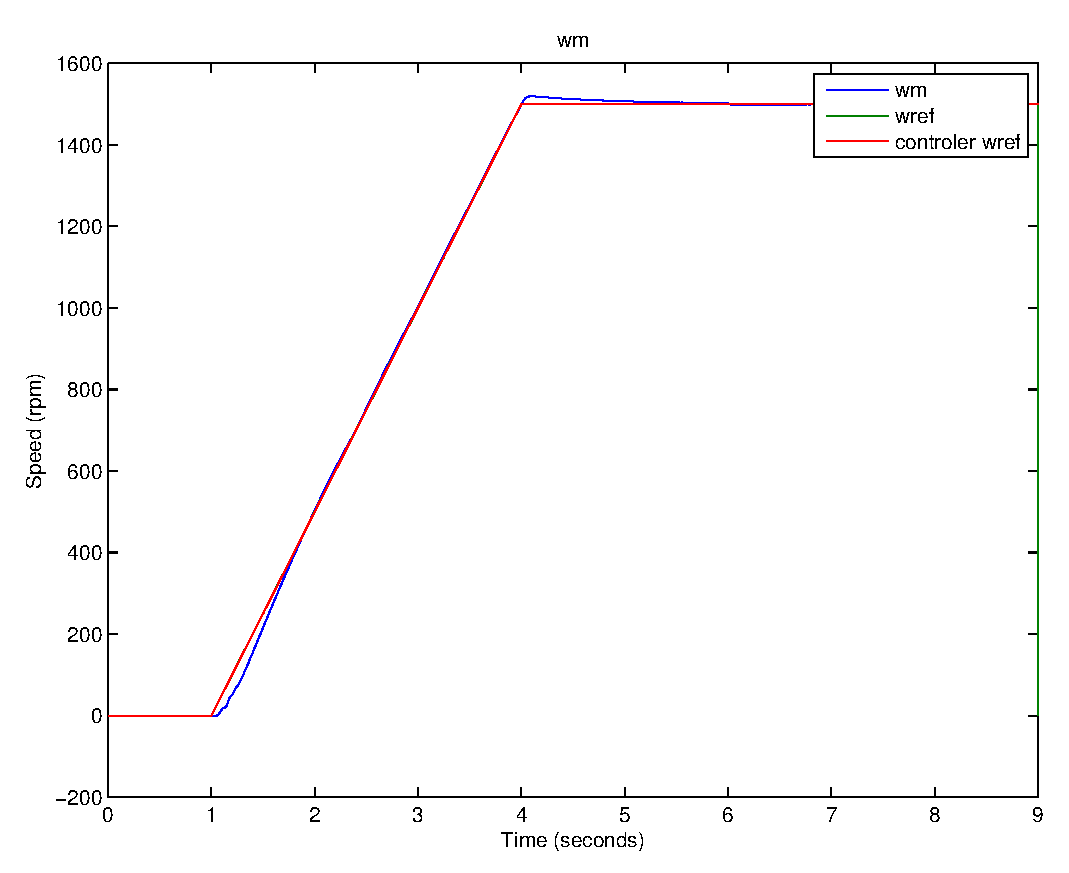
\includegraphics[width=\linewidth]{matlab/wm2}
		\caption{Velocidade Angular}
	\end{subfigure}
	\begin{subfigure}[b]{0.49\linewidth}
		\centering
		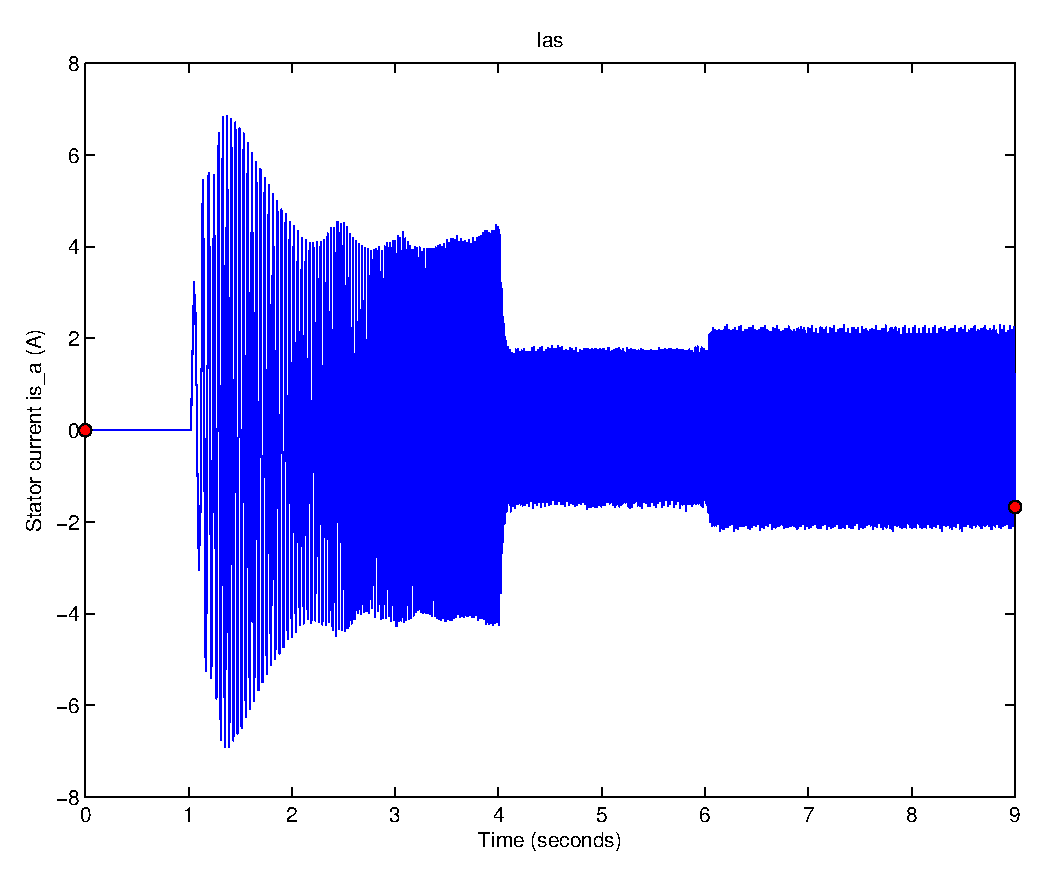
\includegraphics[width=\linewidth]{matlab/ias2}
		\caption{Corrente no estator}
	\end{subfigure}
	\begin{subfigure}[b]{0.49\linewidth}
		\centering
		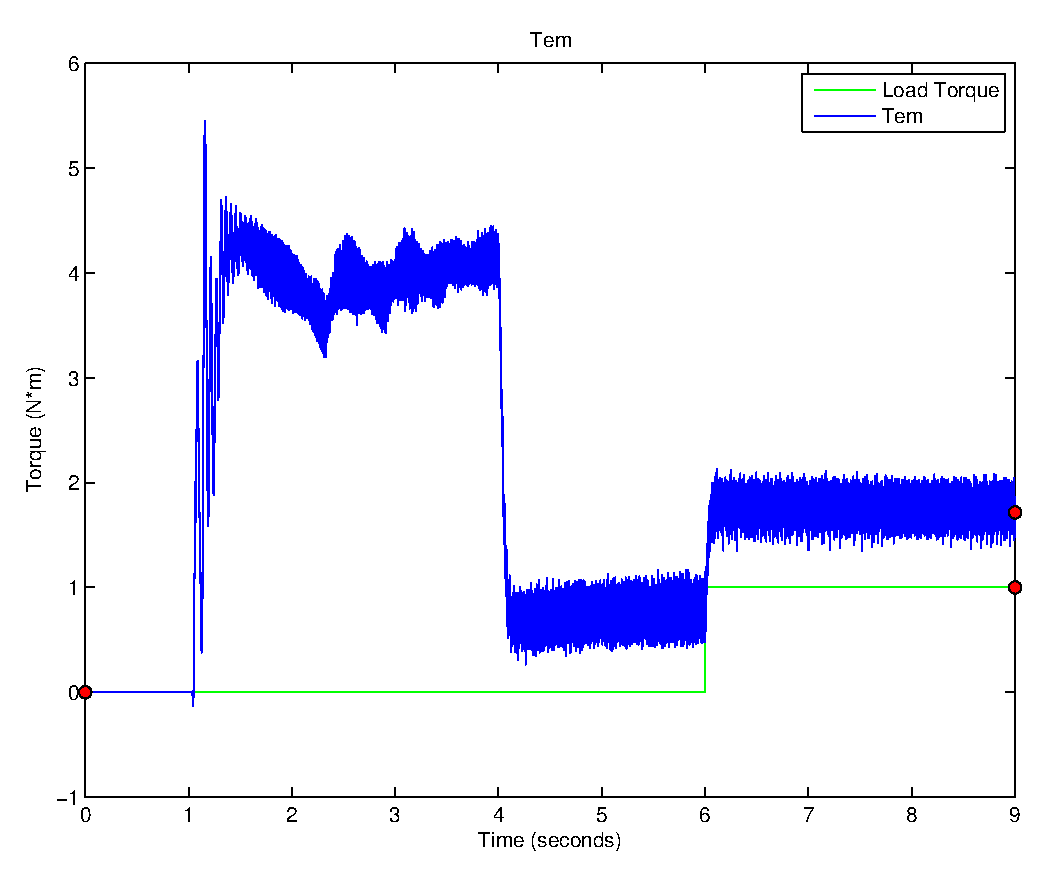
\includegraphics[width=\linewidth]{matlab/tem2}
		\caption{Torque eletromagnético}
	\end{subfigure}
	\begin{subfigure}[b]{0.49\linewidth}
		\centering
		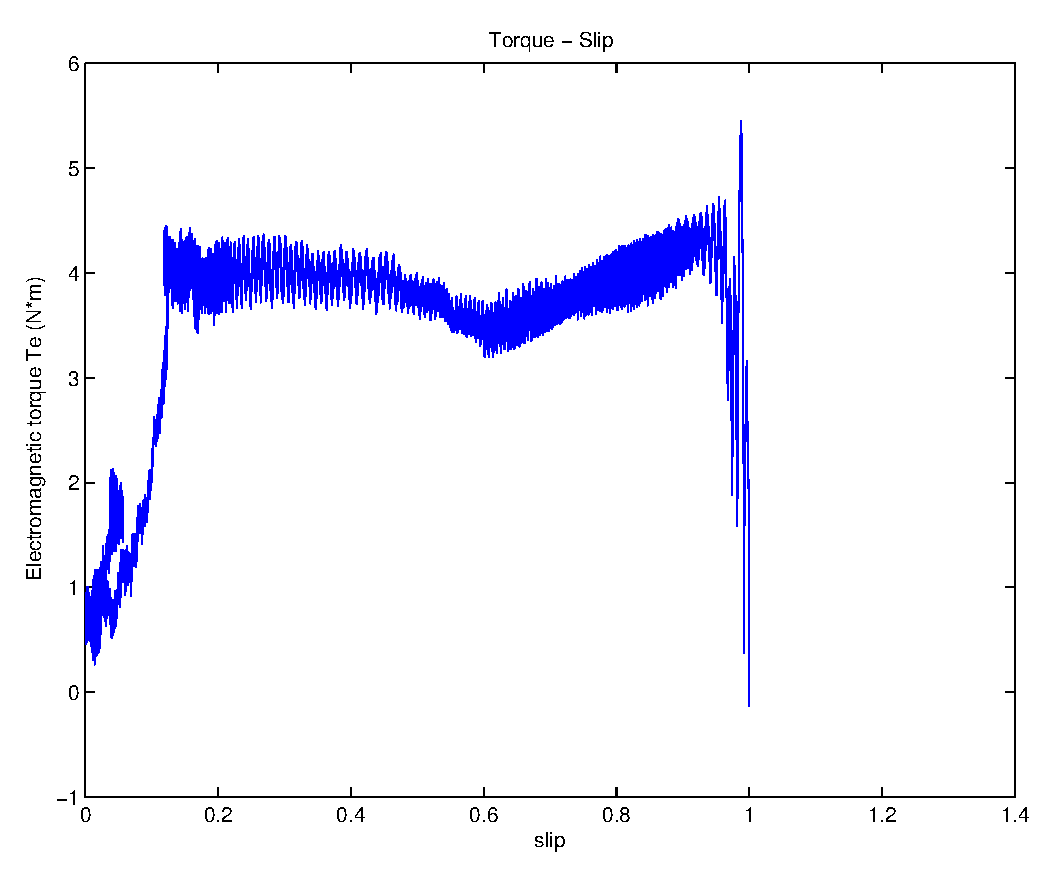
\includegraphics[width=\linewidth]{matlab/ts2}
		\caption{Torque em função do slip}
	\end{subfigure}
	\caption{Curvas de resposta para segunda simulação}
	\label{fig:s2}
\end{figure}

Podemos ver que nosso controlador seguiu perfeitamente a rampa de velocidade, porém a curva de torque não foi muito respeitada. Durante o período de aceleração o torque está longe do desejado o controle só passa a fazer efeito quando a velocidade está estável, nesses momentos nosso controlador apresentou um erro estacionário de aproximadamente $1 N\cdot m$.

%TODO falar do slip, entender graficos

\section{Questões}
\subsection{Efeito do campo girante em máquinas de indução assíncronas trifásicas}
Conforme detalhado em \cite{bb:learneng}, a corrente passando pelas bobinas do estator gera um campo magnético, cada fase do nosso sistema trifásico gera então um campo magnético que varia com o tempo. O campo magnético resultante da soma de todas as fases é um campo de intensidade constante mas orientação variável (cuja velocidade de rotação é chamada de frequência síncrona), o chamado campo girante. O campo girante provoca por sua vez o surgimento de uma corrente no rotor.
Essa corrente induzida no rotor gera um fluxo no entreferro, que gira com a mesma velocidade do rotor, e a interação entre os fluxos causa o torque no sistema. Caso a velocidade do rotor e o fluxo gerado pelo estator possuíssem a mesma frequência, não existiria corrente induzida, logo a velocidade do rotor sempre seria menor do que a frequência síncrona. A diferença entre as velocidades do fluxo gerado no estator e a velocidade do rotor é chamada de escorregamento.
\subsection{Diagrama de blocos da estratégia de controle V-Hz}
% TODO
\subsection{Controle escalar vantagens e desvantagens}
%TODO
\subsection{Controle vetorial}
%TODO
\bibliography{mybib}
\end{document}

